\subsection{Basic functionality}

\begin{note}
Let's suppose we have the following dataset where 
\begin{itemize}
  \item Our target feature has two possible classes: sun and cloud. 
  \item We have two descriptive features: x and y
\end{itemize}

The data set is separable, and our goal is now to find the best hyperplane (a line here) separating the two classes.

\begin{figure}[H]
  \centering
  \begin{subfigure}{0.3\textwidth}
    \centering
    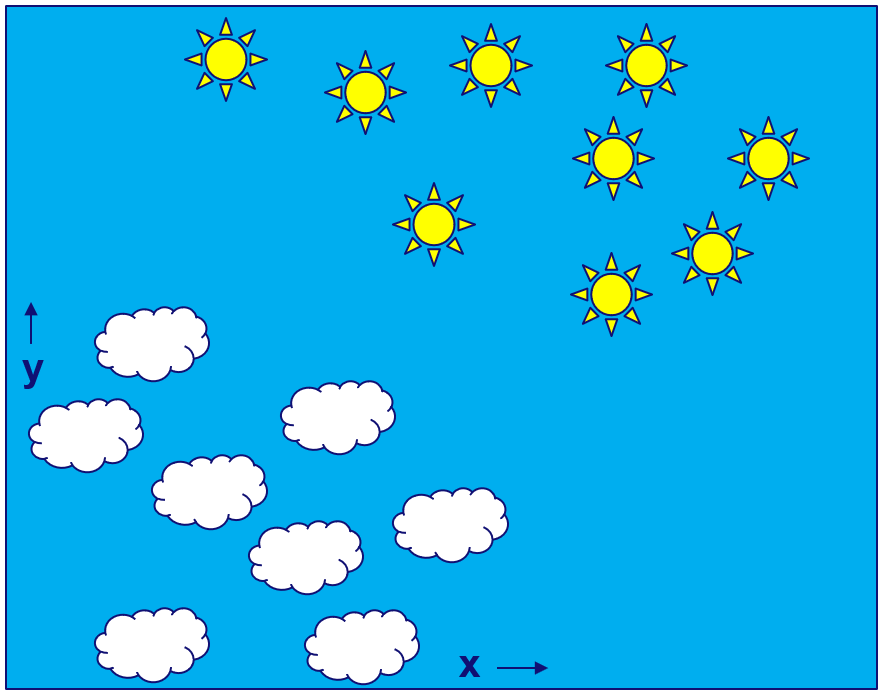
\includegraphics[width=0.8\textwidth]{assets/svm/b__original_set.png}
    \subcaption{Original data set}
  \end{subfigure}\hspace*{0.05\textwidth}
  \begin{subfigure}{0.3\textwidth}
    \centering
    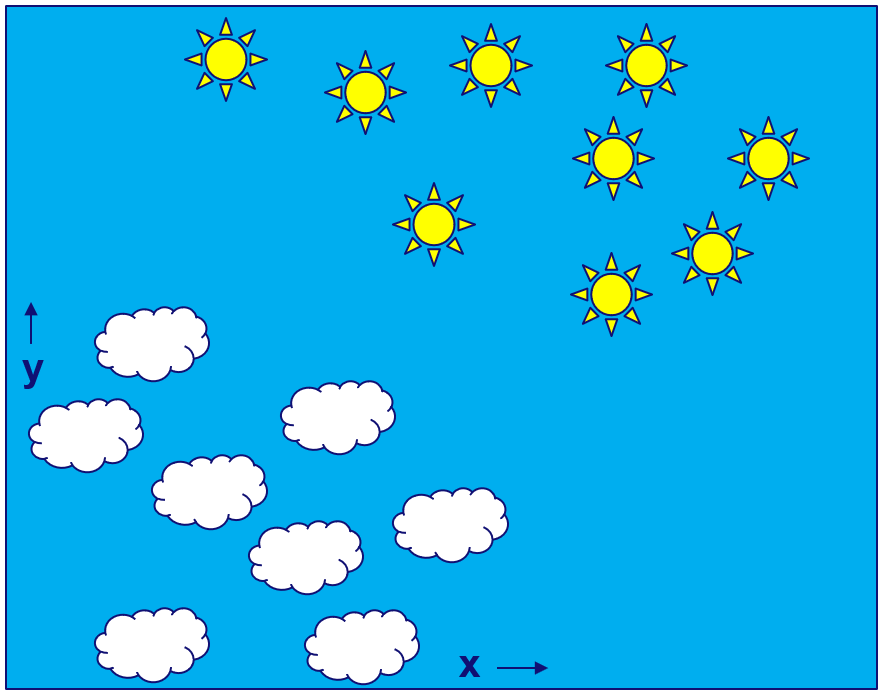
\includegraphics[width=0.8\textwidth]{assets/svm/b__original_set.png}
    \subcaption{Proposal separating lines}
  \end{subfigure}\hspace*{0.05\textwidth}
  \begin{subfigure}{0.3\textwidth}
    \centering
    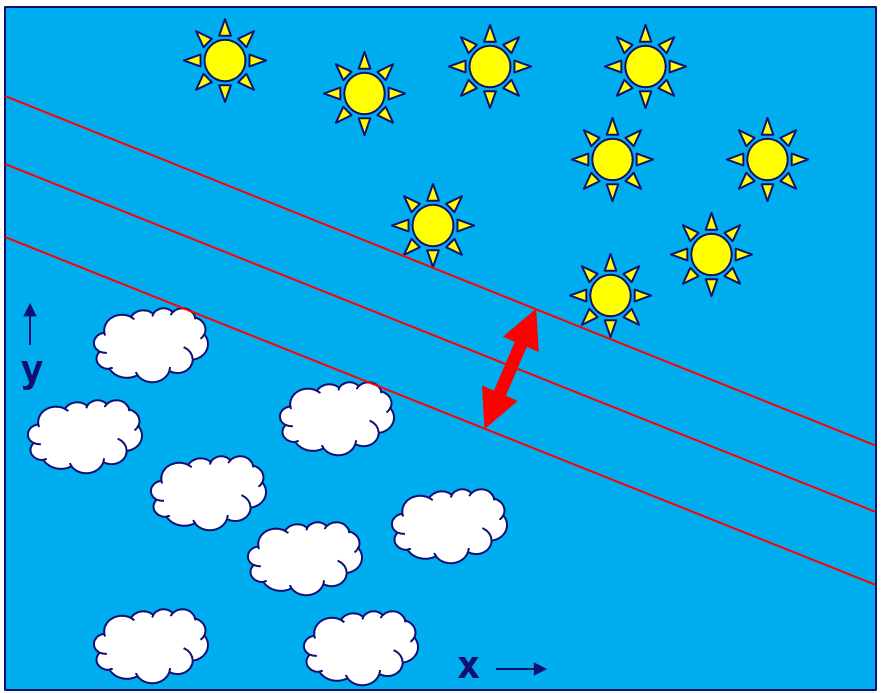
\includegraphics[width=0.8\textwidth]{assets/svm/b__hyperplane_margin.png}
    \subcaption{Line with margin}
  \end{subfigure}
  \caption{Example for SVM}
  \label{fig:5_example_1}
\end{figure}

We need to determine which proposal lines are better than others. The idea to determine this is that the degrees of freedom become less when the separating hyperplane gets thicker. The best hyperplane is:
\begin{itemize}
  \item The best-separating hyperplane is the one fitting between the data points with the maximal thickness (= safety margin).
  \item Therefore, SVMs also tend to be more robust than logistic regression.
\end{itemize}

\end{note}

Consider now a more abstract data set:

\begin{figure}[H]
  \centering
  \begin{subfigure}{0.3\textwidth}
    \centering
    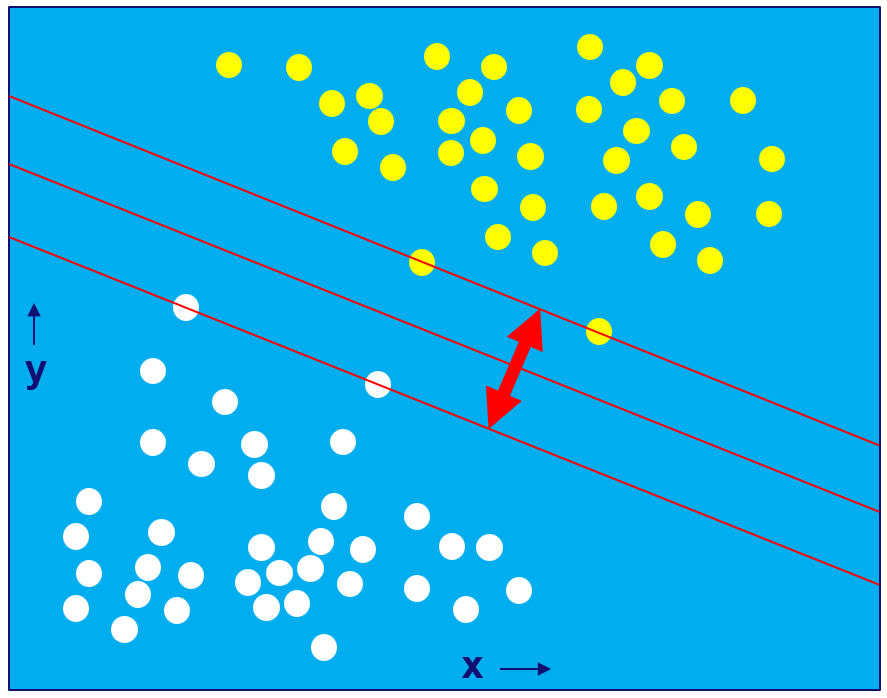
\includegraphics[width=1\textwidth]{assets/svm/b__idea_hyperplane.png} 
    \subcaption{Data set with hyperplane and safety margin}
  \end{subfigure}\hspace*{0.05\textwidth}
  \begin{subfigure}{0.6\textwidth}
    \text{We have instances that are (atomic) points in an $n$-dimensional space.}
  \end{subfigure}
  \vspace*{0.5cm}
  
  \begin{subfigure}{0.3\textwidth}
    \centering
    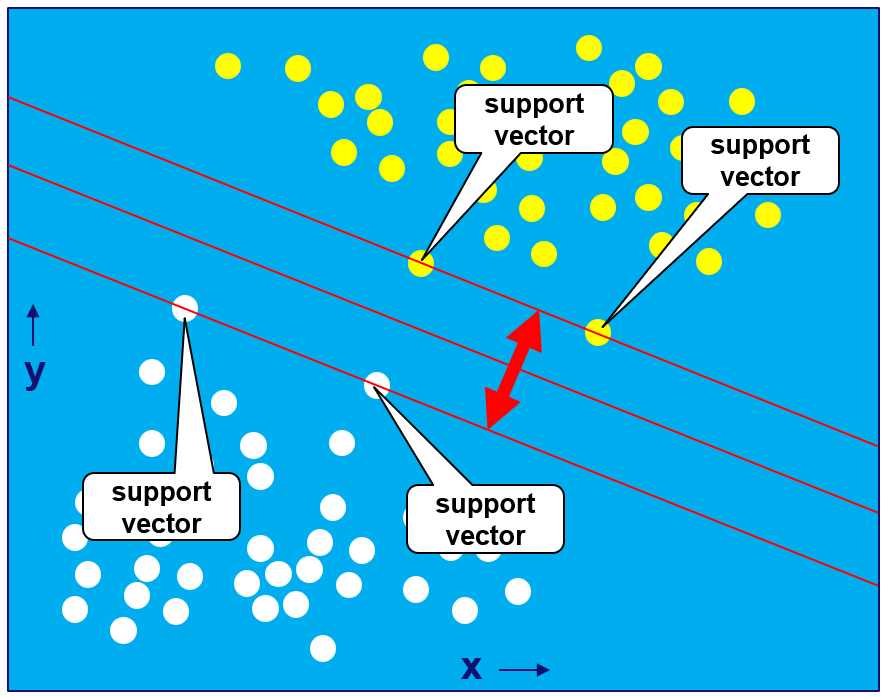
\includegraphics[width=1\textwidth]{assets/svm/b__idea_sv.png} 
    \subcaption{Support vectors}
  \end{subfigure}\hspace*{0.05\textwidth}
  \begin{subfigure}{0.6\textwidth}
    \text{\textbf{Support vectors}\sidenote{Support vector} (SV) are the boundary points $\rightarrow$ only those matter.}
  \end{subfigure}
  \vspace*{0.5cm}
  
  \begin{subfigure}{0.3\textwidth}
    \centering
    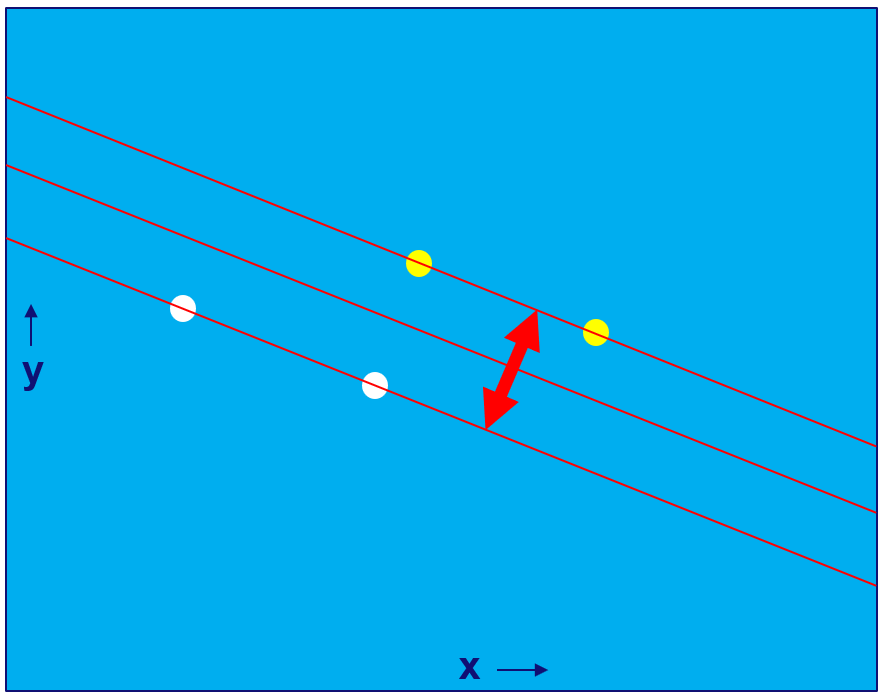
\includegraphics[width=1\textwidth]{assets/svm/b__idea_sv_cleared.png} 
    \subcaption{Reduced problem}
  \end{subfigure}\hspace*{0.05\textwidth}
  \begin{subfigure}{0.6\textwidth}
    \text{Define a \textbf{QP}\sidenote{Quadratic programming} problem (quadratic programming) to make (compared to logistic regression):
    \begin{itemize}
      \item Things more efficient
      \item It less sensitive to outliers
      \item Reduce the risk of overfitting
    \end{itemize}
    But, there are applications where logistic regression works better.}
  \end{subfigure}
  \caption{SVM basic idea}
  \label{fig:5_basic_principle}
\end{figure}

The dimension of the separating hyperplane is always $n-1$ where $n$ is the dimension of the space.
\begin{itemize}
  \item One descriptive feature $\rightarrow$ hyperplane is a point (of dimension $0=n-1$)
  \item Two descriptive features $\rightarrow$ hyperplane is a line (of dimension $1=n-1$)
  \item Three descriptive features $\rightarrow$ hyperplane is a plane (of dimension $2=n-1$)
  \item $\dots$
\end{itemize}

For $n>3$, the problem can't be visualized anymore, but SVMs also work for very large $n$.
\begin{itemize}
  \item This is in contrast to logistic regression, which gets too complex at large $n$
\end{itemize}

The technical definition of the \textbf{hyperplane}\sidenote{Hyperplane} is as follows:
\begin{align*}
  \cv{w} \cdot \cv{x} + b 
  = \underbrace{\mathbf{w}_1\mathbf{x}_1 + \mathbf{w}_2\mathbf{x}_2 + \cdots +\mathbf{w}_n\mathbf{x}_n}_{\begin{array}{c}\scriptstyle\cv{x}=(x_1, x_2, \dots, x_n)\\\scriptstyle\cv{w}=(w_1, w_2, \dots, w_n)\end{array}} + b 
  = 0
\end{align*}

At least one of the weights is non-zero. The hyperplane then splits the $n$-dimensional into two disjoint parts:
\begin{itemize}
  \item $\cv{w} \cdot \cv{x} + b \geq 0$
  \item $\cv{w} \cdot \cv{x} + b < 0$
\end{itemize}

There are some cases where the dataset is not separable. 
\begin{itemize}
  \item This can be due to \textbf{outliers}. A solution for this problem is to relax the problem by allowing violating instances $\rightarrow$ but they then add a penalty.
  \item Alternatively, there can also be a \textbf{structural} problem (not linearly separable in $n$-dimensional space). The idea to solve this problem is to try whether the problem is linearly separable in a higher-dimensional space, which then also includes feature design.
\end{itemize}

We need to make some further definitions to completely formalize the SVM approach. We'll first look at \textbf{vectors}\sidenote{Vector} like $\cv{x} = (x_1, x_2, \dots, x_n)$.
\begin{itemize}
  \item The vector \textbf{length}\sidenote{Vector length} is defined as 
  \begin{align*}\lVert\, \cv{x} \,\lVert = \sqrt{x_1^2 + x_2^2 + \cdots + x_n^2}\end{align*}
  \item The vector \textbf{direction}\sidenote{Vector direction} is the normalized vector of length one, so 
  \begin{align*}\cv{w} = \frac{\cv{x}}{\lVert\, \cv{x} \,\lVert} = \left(\frac{x_1}{\lVert\, \cv{x} \,\lVert}, \frac{x_2}{\lVert\, \cv{x} \,\lVert}, \cdots, \frac{x_n}{\lVert\, \cv{x} \,\lVert}\right)\end{align*}
  \item To extend the length of a vector without changing its direction, multiply the vector with a constant
  \begin{align*}q\cv{x} = (q\cdot x_1, q\cdot x_2, \dots, q\cdot x_n)\end{align*}
  \item The dot product on the other hand allows the multiplication of two vectors: 
  \begin{align*}\cv{x}\cdot\cv{y} = \sum_{i=1}^n x_i y_i = \underbrace{\lVert\, \cv{x} \,\lVert\cdot\lVert\, \cv{y} \,\lVert\cdot \cos \theta}_{\text{with angle }\theta \text{ between }x,y} \in \mathbb{R}\end{align*}
  \begin{note}
    \begin{itemize}
      \item The dot product is heavily influenced by the angle between the two vectors and therefore also tells their linear dependency.
      \item For orthogonal vectors $\cos \theta = 0$, for vectors with the same direction $\cos \theta = 1$ and for angles in the opposite direction $\cos \theta = -1$
    \end{itemize}
  \end{note}
\end{itemize}

Now, let's look deeper into the definition of a hyperplane. Our hyperplane is defined by
\begin{align*}
  \cv{w}\cdot\cv{x} + b = 0 \Longleftrightarrow  \sum_{i=1}^n w_ix_i + b = 0
\end{align*}
where
\begin{itemize}
  \item $\cv{x} = (x_1, x_2, \dots, x_n)$ are free variables,
  \item $\cv{w} = (w_1, w_2, \dots, w_n)$ is the direction vector of the hyperplane (no-zero),
  \item And the hyperplane is fully defined by $\cv{w}$ and $b$
\end{itemize}

Further interesting to see:
\begin{align*}\begin{aligned}
  \text{For } {\color{burntorange}q}\in\mathbb{R}\setminus\{0\}:&&
  \cv{w}\cdot\cv{x} + b = 0 &\Longleftrightarrow  \sum_{i=1}^n w_ix_i + b = 0\\
  \Longleftrightarrow && {\color{burntorange}q}\cv{w}\cdot\cv{x} + {\color{burntorange}q}b = 0 &\Longleftrightarrow  \sum_{i=1}^n {\color{burntorange}q}w_ix_i + {\color{burntorange}q}b = 0
\end{aligned}\end{align*}

The hyperplane splits a set of data points in the following way. Assume we have $N$ data points $X_N = \{\cv{x}_i = (x_{i,1}, x_{i,2}, \dots, x_{i,n})\,|\,i\in N\}$. Then, for $\cv{x}_i$ calculate $f(\cv{x}_i) := \cv{w}\cdot\cv{x}_i + b = \sum_{j=1}^n w_jx_{i, j}+b$, and
\begin{align*}\begin{aligned}
  \text{Classifiy as } 
    \begin{array}{c}\text{positive}\\\text{negative}\end{array} 
  \text{ if } f(\cv{x}_i)
    \begin{array}{c}\geq 0\\< 0\end{array}
\end{aligned}\end{align*}

Note the ongoing confusion of whether above or below the hyperplane is defined as positive, e.g. by multiplying $\cv{w}$ and $b$ with $q=-1$

By splitting the data as described above, we introduce two possible classes for each $\cv{x}_i$, namely $y_i \in \{-1, 1\}$. If our hyperplane $(\cv{w}, b)$ \textbf{separates} a dataset $X_N$ \textbf{perfectly}\sidenote{Perfectly separating hyperplane}, then:
\begin{align*}\begin{aligned}
  \text{For all instances } (\cv{x}_i, y_i):
    \begin{array}{lll}y_i = + 1&\implies&f(\cv{x}_i)\geq 0 \\y_i = - 1&\implies&f(\cv{x}_i) < 0\end{array} 
\end{aligned}\end{align*}

But actually, there might be many "perfect" hyperplanes. The one we would like to pick is the one that maximizes the distance of the hyperplane to the nearest point. For that, we of course first need to define the \textbf{distance between a point and a hyperplane}. Assume, we have the following setting:

\begin{figure}[H]
  \centering
  \begin{subfigure}{0.4\textwidth}
    \centering
    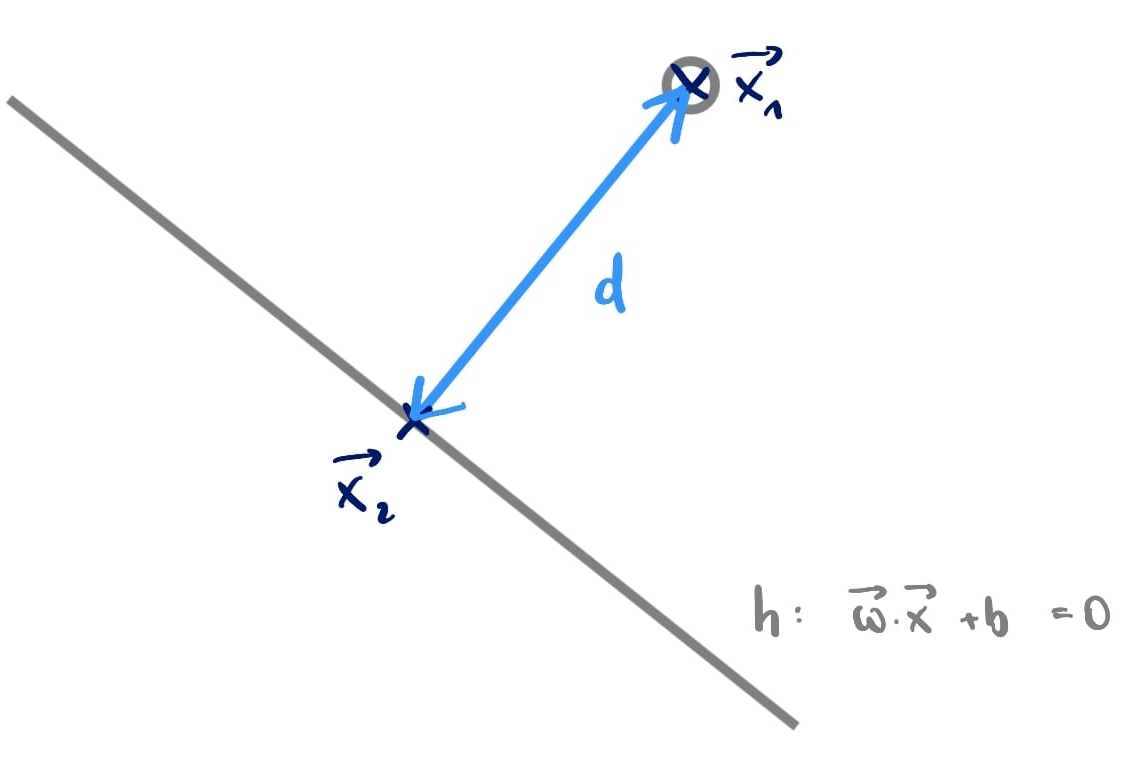
\includegraphics[width=1\textwidth]{assets/svm/b__distance.png} 
  \end{subfigure}\hspace*{0.05\textwidth}
  \begin{subfigure}{0.5\textwidth}
    \text{Assume any point $\cv{x}_1$ and hyperplane $(\cv{w}, b)$}

    \text{
    \begin{itemize}
      \item $\cv{x}_2$ is closest point on the hyperplane
      \item $d$ as distance between $\cv{x}_1$ and the hyperplane, defined as the distance between the two points
    \end{itemize}}
  \end{subfigure}
  \caption{Distance between a point and the hyperplane}
  \label{fig:5_distance_to_h}
\end{figure}

As can be seen in figure \ref{fig:5_distance_to_h}, we have the closest point defined as the point that can be found by following an orthogonal path and seeing which point is on the hyperplane:
\begin{align*}\begin{aligned}
  &\underbrace{\cv{x}_1 = \cv{x}_2 + \lambda \cv{w}}_{\text{orthogonal path}} \text{ and } \underbrace{\cv{w}\cdot\cv{x}_2 + b = 0}_{\cv{x}_2\text{ is on hyperplane}}\\
  \Longrightarrow\quad & \cv{w}\cdot(\cv{x}_1 - \lambda \cv{w}) + b = 0\\
  \Longrightarrow\quad & d = \norm{ \lambda \cv{w} }
\end{aligned}\end{align*}

Next, we try to get rid of the $\lambda$ in the computation of $d = \norm{ \lambda \cv{w} }$. For that, just rewrite the formula for the calculation of $\cv{x}_2$:
\begin{align*}\begin{aligned}
  && \cv{w}\cdot(\cv{x}_1 - \lambda \cv{w}) + b &= 0\\
  \Longrightarrow\quad && \cv{w}\cdot\cv{x}_1 + b &= \lambda \cv{w} \cdot \cv{w} = \lambda \norm{\cv{w}}^2\\
  \Longrightarrow\quad && \lambda  &= \frac{\cv{w}\cdot\cv{x}_1 + b}{\norm{\cv{w}}^2} \\
  \Longrightarrow\quad && d  &= \left|\!\left| \left(\frac{\cv{w}\cdot\cv{x}_1 + b}{\norm{\cv{w}}^2}\right)\cdot\cv{w} \right|\!\right|\\
  &&& = \left| \frac{\cv{w}\cdot\cv{x}_1 + b}{\norm{\cv{w}}^2} \right|\,\norm{\cv{w}} = \left| \frac{\cv{w}\cdot\cv{x}_1 + b}{\norm{\cv{w}}} \right|
\end{aligned}\end{align*}

So finally, we can formulate how to calculate the \textbf{optimal hyperplane}\sidenote{Optimal hyperplane}:
\begin{align*}\begin{aligned}
  \text{Given } \big\{ \left(\cv{x}_i, y_i\right) \in \mathbb{R}^n\times\{-1,1\} \,\big|\, 1\leq i \leq m \big\}\\
  \text{Find } (\cv{w}, b) \text{ such that for any } 1\leq i \leq m:
  &\ \begin{array}{ll}
    \text{If } y_i = +1 & \text{, then } \cv{w}\cdot\cv{x}_i + b \geq 0\\
    \text{If } y_i = -1 & \text{, then } \cv{w}\cdot\cv{x}_i + b < 0
  \end{array}\\
  \text{And maximize } \min {}_{1\leq i<m}d_i \text{ with}:
  &\ \ \,d_i = \left| \frac{\cv{w}\cdot\cv{x}_i + b}{\norm{\cv{w}}} \right|
\end{aligned}\end{align*}

Alternatively, we could normalize the distance to one, such that the resulting situation is as depicted in \ref{fig:5_distance_to_h_normalized}.
\begin{itemize}
  \item This rescaling can be performed since the hyperplane formulation doesn't change when multiplying with a constant $q$.
  \item The support vectors yield the result $\cv{w}\cdot\cv{x}_i + b = \pm 1$.
\end{itemize}

\begin{figure}[H]
  \centering
  \begin{subfigure}{0.4\textwidth}
    \centering
    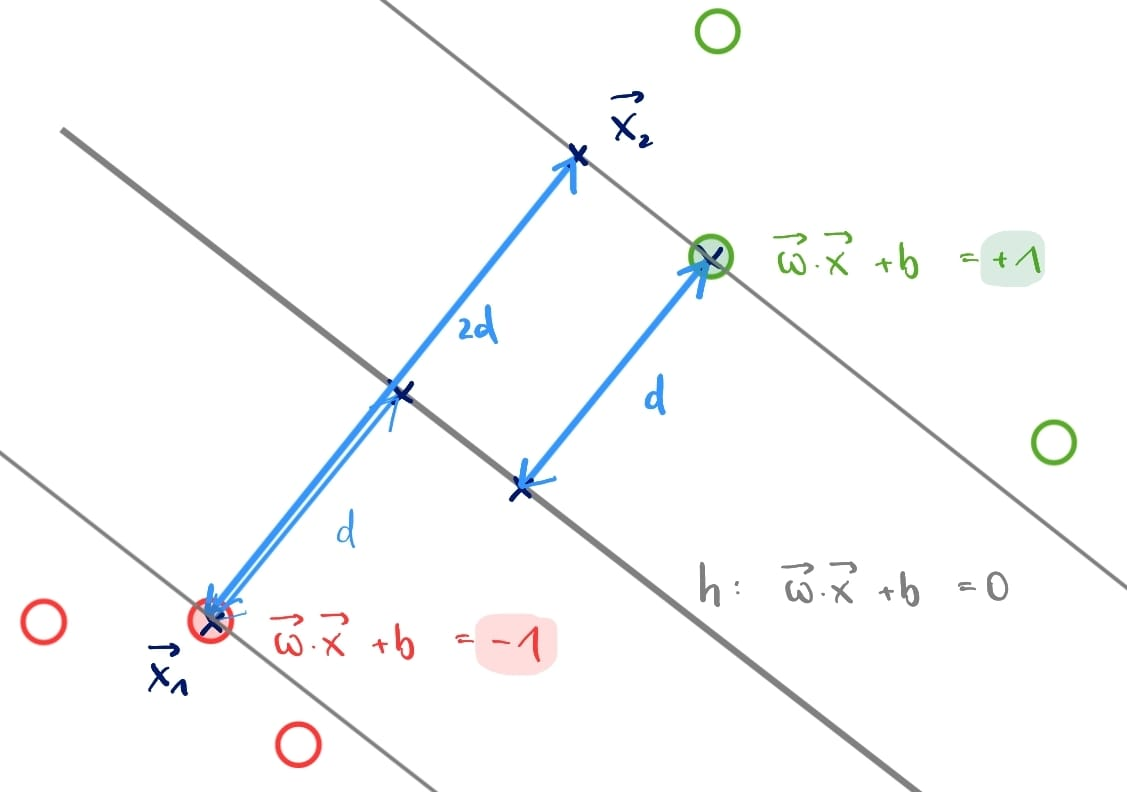
\includegraphics[width=1\textwidth]{assets/svm/b__distance_1.png} 
  \end{subfigure}\hspace*{0.05\textwidth}
  \begin{subfigure}{0.5\textwidth}
    \text{The support vectors are on the lines}

    \text{\color{gray}(positive and negative support vectors)}
  \end{subfigure}
  \caption{Normalized distance}
  \label{fig:5_distance_to_h_normalized}
\end{figure}

Also, the classification is adjusted to 
\begin{align*}
  \left.\begin{array}{ll}
    \text{If } y_i = +1 & \text{, then } \cv{w}\cdot\cv{x}_i + b \geq +1\\
    \text{If } y_i = -1 & \text{, then } \cv{w}\cdot\cv{x}_i + b \leq -1
  \end{array}\right\}
  \begin{array}{ll}\rightarrow&\text{can be combined to:}\\
    &\forall i: y_i(\cv{w}\cdot\cv{x}_i + b) \geq 1\sidenote{Optimal hyperplane normalized}
  \end{array}
\end{align*}

Our goal is still to maximize the smallest $d=\norm{\lambda \cv{w}}$. In our alternative formulation, we want to formalize this goal only with the help of the shifted hyperplanes $\cv{x}\cdot\cv{x} + b = \pm1$:
\begin{itemize}
  \item Choose an arbitrary support vector $\cv{x}_1$ \begin{note}(let's say on $\cv{x}\cdot\cv{x} + b = -1$)\end{note}
  \item Now take the corresponding $\cv{x}_2 = \cv{x}_1 + 2\lambda\cv{w}$ on the other support-vector-line \begin{note}(so $\cv{w}\cdot\cv{x} + b = +1$)\end{note}
  \item This leads to the following equations to be solved:
  \begin{align*}\begin{aligned}
    \cv{w}\cdot\cv{x}_1 + b &= -1 \\
    \cv{w}\cdot(\cv{x}_1 + 2\lambda\cv{w}) + b &= +1
  \end{aligned}\end{align*}
  \item This can be further readjusted to:
  \begin{align*}\begin{aligned}
    \implies && \underbrace{\cv{w}\cdot\cv{x}_1 + b}_{=-1} + \cv{w}\cdot2\lambda\cv{w} &= +1\\
    \implies && \cv{w}\cdot2\lambda\cv{w} &= +2\\
    \implies && \lambda &= \frac{1}{\cv{w}\cdot\cv{w}} = \frac{1}{\norm{\cv{w}}^2}
  \end{aligned}\end{align*}
  \item So, we can replace:
  \begin{align*}
    &\text{Maximize } d=\norm{\lambda \cv{w}} = \frac{1}{\norm{\cv{w}}^2}\norm{\cv{w}} = \frac{1}{\norm{\cv{w}}}\\
    &\text{Minimize } \norm{\cv{w}} \text{ \begin{note} under the constraints stated before\end{note}}
  \end{align*}
\end{itemize}

So, the reformulated problem is:
\begin{align*}\begin{aligned}
  \text{Given a set of } m \text{ instances }& \big\{ (\cv{x}_i, y_i) \in \mathbb{R}^n\times\{-1,1\} \,\big|\, 1\leq i\leq m \big\}\sidenote{Reformulated: SVM problem}\\
  \min_{\cv{w}, b}\norm{\cv{w}} \text{ s.t. }& \forall i: y_i(\cv{w}\cdot\cv{x}_i + b) \geq 1
\end{aligned}\end{align*}

For technical reasons, a common variant of this problem is the convex quadratic optimization problem
\begin{align*}\begin{aligned}
  \text{Given a set of } m \text{ instances }&\big\{ (\cv{x}_i, y_i) \in \mathbb{R}^n\times\{-1,1\} \,\big|\, 1\leq i\leq m \big\}\sidenote{Convex quadratic optimization problem}\\
  \min_{\cv{w}, b}\frac{1}{2}\norm{\cv{w}}^2 \text{ s.t. }& \forall i: y_i(\cv{w}\cdot\cv{x}_i + b) \geq 1
\end{aligned}\end{align*}
\begin{itemize}
  \item This problem is easier to solve than the original linear formulation (maximizing $\min_{1\leq i<m}d_i$)
  \item The concrete solution or techniques for finding solutions are not covered here, but assume they exist
\end{itemize}

Another reformulation of the problem is the Wolfe dual Lagrangian problem which is important for the "kernel trick":
\begin{align*}\begin{aligned}
  &\text{For } \cv{w}=\sum_{i=1}^m \alpha_i y_i \cv{x}_i \text{ and } \alpha_i\geq0, i=1,\dots,m \sidenote{Wolfe dual Lagrangian problem}\\
  & \begin{array}{rl}
      \max_\alpha & \sum_{i=1}^m \alpha_i - \frac{1}{2} \sum_{i=1}^m \sum_{j=1}^m \alpha_i \alpha_j y_i y_j \cv{x}_i\cv{x}_j\\
      \text{subject to } & \sum_{i=1}^m \alpha_i y_i = 0
  \end{array}
\end{aligned}\end{align*}

